% About Unity

\section{External Assets}
\label{sec:external_assets}
\import{}{external_assets.tex}

% \section{The architecture}
\begin{figure}%[h!] %[H]
	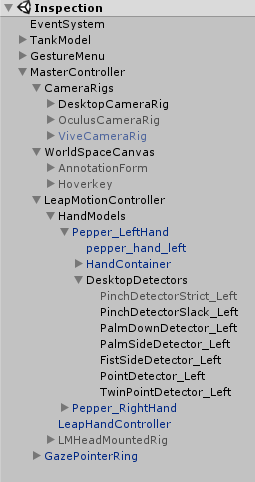
\includegraphics{pictures/unity_hierarchy.png} % Create a better hierarchical view?
	\caption[The Unity project hierarchy of the Design Review Application]{The Unity project hierarchy of the Design Review Application}
	\label{fig:unity_hierarchy}
\end{figure} 

The Unity project has four top-level game objects: \texttt{EventSystem}, \texttt{TankModel}, \texttt{GestureMenu} and \texttt{MasterController}. 
%as visible in~\vref{fig:unity_hierarchy}. 

The \texttt{EventSystem} game object is responsible for processing and handling events and input actions in the scene. 
In this implementation a standard unity event system is used (generated when creating a new systems), with some modifications done for virtual reality.
Most of these modification are accomplished by the \texttt{OVRInputModule} script, which inspired by an Oculus VR sample project. 
Apart from this no other changes was done to \texttt{EventSystem} as it worked optimally "right out of the box".

The \texttt{TankModel} game object contains several child objects that together make up the oiltank-model, which this application is based on.
Originally the design included the functionality to load different models into the application and starts sessions, but 
this was fell out of scope to both prioritize the gesture recognition and virtual reality aspect, and because of a low availability of similar models.
The tank model has not received any changes during implementation and has been used as it was supplied. 

The \texttt{GestureMenu} and \texttt{MasterController} together contain most of the key components of the application and they and their child objects will
be the focus for the rest of this chapter. \texttt{GestureMenu} represents the gesture menu, which by default is available by directing the left hand palm in the 
direction of the camera. The \texttt{MasterController} game object represents the player model and contains many of the most important game objects, in addition to
holding many key scripts. The \texttt{MasterController}'s transform, with its position, rotation and scale, represents the user's position and orientation, 
and every child object of \texttt{MasterController} will have a position, rotation and scale that is relative to its own. This ensures
that e.g.~the camera will always "follow" the user. Several of the important game objects that are covered in later sections are children of 
the master controller for this reason. First, however, we will cover the important components of \texttt{MasterController}.

\begin{figure}%[h!] %[H]
	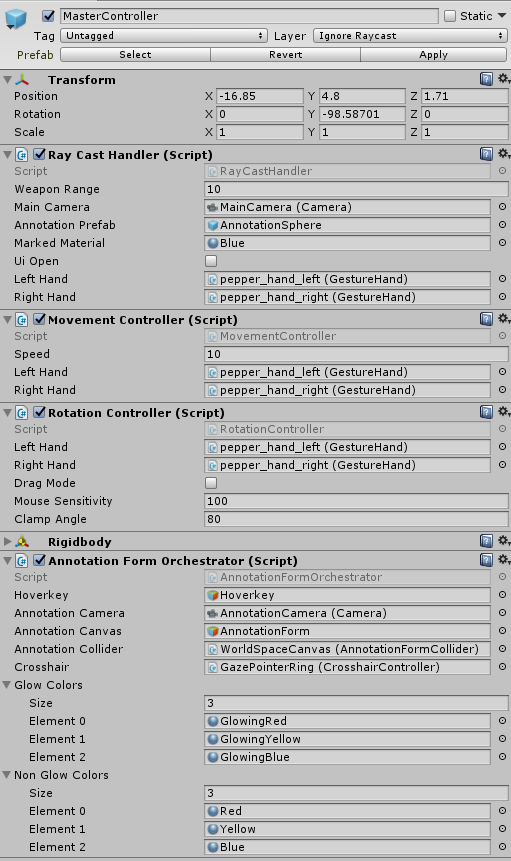
\includegraphics{pictures/unity_inspector.png} % Get better resolution?
	\caption[The \texttt{MasterController} components]{The \texttt{MasterController} components seen in the Unity Inspector view.}
	\label{fig:unity_inspector}
\end{figure} 

\section{The Master Controller Components}
\import{}{master_controller_components.tex}


\section{The Camera Rigs}
\label{sec:camera_rigs}
\import{}{camera_rigs.tex}


\section{The World Space Canvas}
\label{sec:world_space_canvas}
\import{}{world_space_canvas.tex}


\section{The Leap Motion Controller}
\label{sec:leap_motion_controller}
\import{}{leap_motion_controller.tex}


\section{The Gesture Hand Class}
\label{sec:gesturehand_class}
\import{}{gesturehand_class.tex}
 

\section{The Detectors}
\label{sec:detectors}
\import{}{detectors.tex}


\section{The Menu}
\label{sec:menu}
\import{}{menu.tex}


\section{The Annotations}
\label{sec:annotations}
\import{}{annotations.tex}


